% Options for packages loaded elsewhere
\PassOptionsToPackage{unicode}{hyperref}
\PassOptionsToPackage{hyphens}{url}
%
\documentclass[
]{article}
\usepackage{amsmath,amssymb}
\usepackage{iftex}
\ifPDFTeX
  \usepackage[T1]{fontenc}
  \usepackage[utf8]{inputenc}
  \usepackage{textcomp} % provide euro and other symbols
\else % if luatex or xetex
  \usepackage{unicode-math} % this also loads fontspec
  \defaultfontfeatures{Scale=MatchLowercase}
  \defaultfontfeatures[\rmfamily]{Ligatures=TeX,Scale=1}
\fi
\usepackage{lmodern}
\ifPDFTeX\else
  % xetex/luatex font selection
\fi
% Use upquote if available, for straight quotes in verbatim environments
\IfFileExists{upquote.sty}{\usepackage{upquote}}{}
\IfFileExists{microtype.sty}{% use microtype if available
  \usepackage[]{microtype}
  \UseMicrotypeSet[protrusion]{basicmath} % disable protrusion for tt fonts
}{}
\makeatletter
\@ifundefined{KOMAClassName}{% if non-KOMA class
  \IfFileExists{parskip.sty}{%
    \usepackage{parskip}
  }{% else
    \setlength{\parindent}{0pt}
    \setlength{\parskip}{6pt plus 2pt minus 1pt}}
}{% if KOMA class
  \KOMAoptions{parskip=half}}
\makeatother
\usepackage{xcolor}
\usepackage[margin=1in]{geometry}
\usepackage{color}
\usepackage{fancyvrb}
\newcommand{\VerbBar}{|}
\newcommand{\VERB}{\Verb[commandchars=\\\{\}]}
\DefineVerbatimEnvironment{Highlighting}{Verbatim}{commandchars=\\\{\}}
% Add ',fontsize=\small' for more characters per line
\usepackage{framed}
\definecolor{shadecolor}{RGB}{248,248,248}
\newenvironment{Shaded}{\begin{snugshade}}{\end{snugshade}}
\newcommand{\AlertTok}[1]{\textcolor[rgb]{0.94,0.16,0.16}{#1}}
\newcommand{\AnnotationTok}[1]{\textcolor[rgb]{0.56,0.35,0.01}{\textbf{\textit{#1}}}}
\newcommand{\AttributeTok}[1]{\textcolor[rgb]{0.13,0.29,0.53}{#1}}
\newcommand{\BaseNTok}[1]{\textcolor[rgb]{0.00,0.00,0.81}{#1}}
\newcommand{\BuiltInTok}[1]{#1}
\newcommand{\CharTok}[1]{\textcolor[rgb]{0.31,0.60,0.02}{#1}}
\newcommand{\CommentTok}[1]{\textcolor[rgb]{0.56,0.35,0.01}{\textit{#1}}}
\newcommand{\CommentVarTok}[1]{\textcolor[rgb]{0.56,0.35,0.01}{\textbf{\textit{#1}}}}
\newcommand{\ConstantTok}[1]{\textcolor[rgb]{0.56,0.35,0.01}{#1}}
\newcommand{\ControlFlowTok}[1]{\textcolor[rgb]{0.13,0.29,0.53}{\textbf{#1}}}
\newcommand{\DataTypeTok}[1]{\textcolor[rgb]{0.13,0.29,0.53}{#1}}
\newcommand{\DecValTok}[1]{\textcolor[rgb]{0.00,0.00,0.81}{#1}}
\newcommand{\DocumentationTok}[1]{\textcolor[rgb]{0.56,0.35,0.01}{\textbf{\textit{#1}}}}
\newcommand{\ErrorTok}[1]{\textcolor[rgb]{0.64,0.00,0.00}{\textbf{#1}}}
\newcommand{\ExtensionTok}[1]{#1}
\newcommand{\FloatTok}[1]{\textcolor[rgb]{0.00,0.00,0.81}{#1}}
\newcommand{\FunctionTok}[1]{\textcolor[rgb]{0.13,0.29,0.53}{\textbf{#1}}}
\newcommand{\ImportTok}[1]{#1}
\newcommand{\InformationTok}[1]{\textcolor[rgb]{0.56,0.35,0.01}{\textbf{\textit{#1}}}}
\newcommand{\KeywordTok}[1]{\textcolor[rgb]{0.13,0.29,0.53}{\textbf{#1}}}
\newcommand{\NormalTok}[1]{#1}
\newcommand{\OperatorTok}[1]{\textcolor[rgb]{0.81,0.36,0.00}{\textbf{#1}}}
\newcommand{\OtherTok}[1]{\textcolor[rgb]{0.56,0.35,0.01}{#1}}
\newcommand{\PreprocessorTok}[1]{\textcolor[rgb]{0.56,0.35,0.01}{\textit{#1}}}
\newcommand{\RegionMarkerTok}[1]{#1}
\newcommand{\SpecialCharTok}[1]{\textcolor[rgb]{0.81,0.36,0.00}{\textbf{#1}}}
\newcommand{\SpecialStringTok}[1]{\textcolor[rgb]{0.31,0.60,0.02}{#1}}
\newcommand{\StringTok}[1]{\textcolor[rgb]{0.31,0.60,0.02}{#1}}
\newcommand{\VariableTok}[1]{\textcolor[rgb]{0.00,0.00,0.00}{#1}}
\newcommand{\VerbatimStringTok}[1]{\textcolor[rgb]{0.31,0.60,0.02}{#1}}
\newcommand{\WarningTok}[1]{\textcolor[rgb]{0.56,0.35,0.01}{\textbf{\textit{#1}}}}
\usepackage{longtable,booktabs,array}
\usepackage{calc} % for calculating minipage widths
% Correct order of tables after \paragraph or \subparagraph
\usepackage{etoolbox}
\makeatletter
\patchcmd\longtable{\par}{\if@noskipsec\mbox{}\fi\par}{}{}
\makeatother
% Allow footnotes in longtable head/foot
\IfFileExists{footnotehyper.sty}{\usepackage{footnotehyper}}{\usepackage{footnote}}
\makesavenoteenv{longtable}
\usepackage{graphicx}
\makeatletter
\def\maxwidth{\ifdim\Gin@nat@width>\linewidth\linewidth\else\Gin@nat@width\fi}
\def\maxheight{\ifdim\Gin@nat@height>\textheight\textheight\else\Gin@nat@height\fi}
\makeatother
% Scale images if necessary, so that they will not overflow the page
% margins by default, and it is still possible to overwrite the defaults
% using explicit options in \includegraphics[width, height, ...]{}
\setkeys{Gin}{width=\maxwidth,height=\maxheight,keepaspectratio}
% Set default figure placement to htbp
\makeatletter
\def\fps@figure{htbp}
\makeatother
\setlength{\emergencystretch}{3em} % prevent overfull lines
\providecommand{\tightlist}{%
  \setlength{\itemsep}{0pt}\setlength{\parskip}{0pt}}
\setcounter{secnumdepth}{5}
\newlength{\cslhangindent}
\setlength{\cslhangindent}{1.5em}
\newlength{\csllabelwidth}
\setlength{\csllabelwidth}{3em}
\newlength{\cslentryspacingunit} % times entry-spacing
\setlength{\cslentryspacingunit}{\parskip}
\newenvironment{CSLReferences}[2] % #1 hanging-ident, #2 entry spacing
 {% don't indent paragraphs
  \setlength{\parindent}{0pt}
  % turn on hanging indent if param 1 is 1
  \ifodd #1
  \let\oldpar\par
  \def\par{\hangindent=\cslhangindent\oldpar}
  \fi
  % set entry spacing
  \setlength{\parskip}{#2\cslentryspacingunit}
 }%
 {}
\usepackage{calc}
\newcommand{\CSLBlock}[1]{#1\hfill\break}
\newcommand{\CSLLeftMargin}[1]{\parbox[t]{\csllabelwidth}{#1}}
\newcommand{\CSLRightInline}[1]{\parbox[t]{\linewidth - \csllabelwidth}{#1}\break}
\newcommand{\CSLIndent}[1]{\hspace{\cslhangindent}#1}
% Load necessary packages
\usepackage{amsmath}    % For advanced math typesetting
\usepackage{graphicx}   % For including images
\usepackage{hyperref}   % For hyperlinks
\usepackage{geometry}   % For setting page dimensions
\usepackage{fancyhdr}   % For custom headers and footers
\usepackage{setspace}   % For setting line spacing

% Set page dimensions
\geometry{
  a4paper,
  left=25mm,
  right=25mm,
  top=25mm,
  bottom=25mm
}

% Custom header and footer
\pagestyle{fancy}
\fancyhf{}
\fancyhead[L]{\leftmark}
\fancyhead[R]{\thepage}

% Custom commands
\newcommand{\HRule}{\rule{\linewidth}{0.5mm}}

% Set line spacing
\setstretch{1.5}

% Additional settings
\hypersetup{
  colorlinks=true,
  linkcolor=blue,
  filecolor=magenta,
  urlcolor=cyan,
  pdftitle={Your Document Title},
  pdfpagemode=FullScreen,
}
\ifLuaTeX
  \usepackage{selnolig}  % disable illegal ligatures
\fi
\IfFileExists{bookmark.sty}{\usepackage{bookmark}}{\usepackage{hyperref}}
\IfFileExists{xurl.sty}{\usepackage{xurl}}{} % add URL line breaks if available
\urlstyle{same}
\hypersetup{
  pdftitle={Lecture 9: Model fitting},
  pdfauthor={Dr Peter E McKenna},
  hidelinks,
  pdfcreator={LaTeX via pandoc}}

\title{Lecture 9: Model fitting}
\usepackage{etoolbox}
\makeatletter
\providecommand{\subtitle}[1]{% add subtitle to \maketitle
  \apptocmd{\@title}{\par {\large #1 \par}}{}{}
}
\makeatother
\subtitle{C91AR: Advanced Statistics using R}
\author{Dr Peter E McKenna}
\date{2025-03-21}

\begin{document}
\maketitle

{
\setcounter{tocdepth}{2}
\tableofcontents
}
\hypertarget{session-outline}{%
\section{Session outline}\label{session-outline}}

\begin{itemize}
\tightlist
\item
  Today, we are going to examine methods for checking how well a model
  fits the data
\item
  We are going to look at a few today outlined in Canduela and Raeside
  (2020)
\item
  Discuss multicollinearity and how to check for it
\item
  On Thursday I will run a code clinic where you can ask me any
  questions about R, to give you some extra support as your prepare the
  summative assessment.
\end{itemize}

\hypertarget{reproducibility-notation}{%
\section{Reproducibility \& notation}\label{reproducibility-notation}}

\begin{Shaded}
\begin{Highlighting}[]
\CommentTok{\# Set seed for reproducibility}
\FunctionTok{set.seed}\NormalTok{(}\DecValTok{123}\NormalTok{)}

\CommentTok{\# Change the output format}
\FunctionTok{options}\NormalTok{(}\AttributeTok{scipen =} \DecValTok{999}\NormalTok{)}
\end{Highlighting}
\end{Shaded}

\hypertarget{load-packages}{%
\section{Load packages}\label{load-packages}}

\begin{Shaded}
\begin{Highlighting}[]
\CommentTok{\# Load packages}
\NormalTok{pacman}\SpecialCharTok{::}\FunctionTok{p\_load}\NormalTok{(tidyverse,}
\NormalTok{               corrr,}
\NormalTok{               tidyplots,}
\NormalTok{               car) }\CommentTok{\# for VIF}
\end{Highlighting}
\end{Shaded}

\hypertarget{data-setup}{%
\section{Data setup}\label{data-setup}}

\begin{Shaded}
\begin{Highlighting}[]
\CommentTok{\# Read in the data}
\NormalTok{handw }\OtherTok{\textless{}{-}}
  \FunctionTok{read\_csv}\NormalTok{(}\StringTok{"data\_raw/heights\_and\_weights.csv"}\NormalTok{,}
           \AttributeTok{col\_types =} \StringTok{"dd"}\NormalTok{)}


\CommentTok{\# Add log transformed vectors to dataset}
\NormalTok{handw\_log }\OtherTok{\textless{}{-}}
\NormalTok{  handw }\SpecialCharTok{|\textgreater{}}
  \FunctionTok{mutate}\NormalTok{(}\AttributeTok{hlog =} \FunctionTok{log}\NormalTok{(height\_in),  }
         \AttributeTok{wlog =} \FunctionTok{log}\NormalTok{(weight\_lbs))}

\CommentTok{\# load grades data for VIF}
\NormalTok{grades }\OtherTok{\textless{}{-}}
  \FunctionTok{read\_csv}\NormalTok{(}\StringTok{"data\_tidy/grades.csv"}\NormalTok{,}
           \AttributeTok{col\_types =} \StringTok{"ddii"}\NormalTok{)}
\end{Highlighting}
\end{Shaded}

\hypertarget{r2-coefficient-of-determination}{%
\section{\texorpdfstring{\(R^{2}\) Coefficient of
determination}{R\^{}\{2\} Coefficient of determination}}\label{r2-coefficient-of-determination}}

\begin{itemize}
\item
  To this point we have created a regression equation and used it to
  predict someone's weight given their height.
\item
  But, we also want to know how good a fit our equation is given the
  data. To calculate this we use the \textbf{\emph{coefficient of
  determination}} (\(R^2\)):
\end{itemize}

\(R^2 = \frac{\text{Sum of Squares Explained by Regression (SSR)}}{\text{Total Sum of Squares (before regression)(TSS)}} = \frac{\underset{i=1}{\stackrel{n}{\sum}}(\hat{y}_{i} - \overline{y})^2}{\underset{i=1}{\stackrel{n}{\sum}}(y_{i} - \overline{y})^{2}}\)

\hypertarget{calculating-the-total-sum-of-squares}{%
\section{Calculating the total sum of
squares}\label{calculating-the-total-sum-of-squares}}

\begin{itemize}
\tightlist
\item
  The total sum of squares (TSS) in the dependent variable (i.e.,
  weight) is split into two parts:

  \begin{itemize}
  \tightlist
  \item
    the part explained by sum of squares explain by regression (SSR),
    which is the sum of the squared differences between the predicted
    values (\(\hat{y}_{i}\)) and the mean of the response variable
    (\(\overline{y}\))
  \end{itemize}
\end{itemize}

\[\text{Sum of Squares Explained by Regression (SSR)} = \sum_{i=1}^{n} (\hat{y}_{i} - \overline{y})^2\]

\begin{itemize}
\tightlist
\item
  the part that is unexplained sum of squared errors (SSE), which is the
  squared difference between the observed values (\(y_{i}\)) and the
  predicted values (\(\hat{y}_{i}\)), since the relationship is never
  perfect and there are always some residuals.
\end{itemize}

\[\text{Sum of Squares Errors (SSE)} = \sum_{i=1}^{n} (y_{i} - \overline{y})^2\]

\hypertarget{where-the-r2-values-come-from}{%
\section{\texorpdfstring{Where the \(R^2\) values come
from}{Where the R\^{}2 values come from}}\label{where-the-r2-values-come-from}}

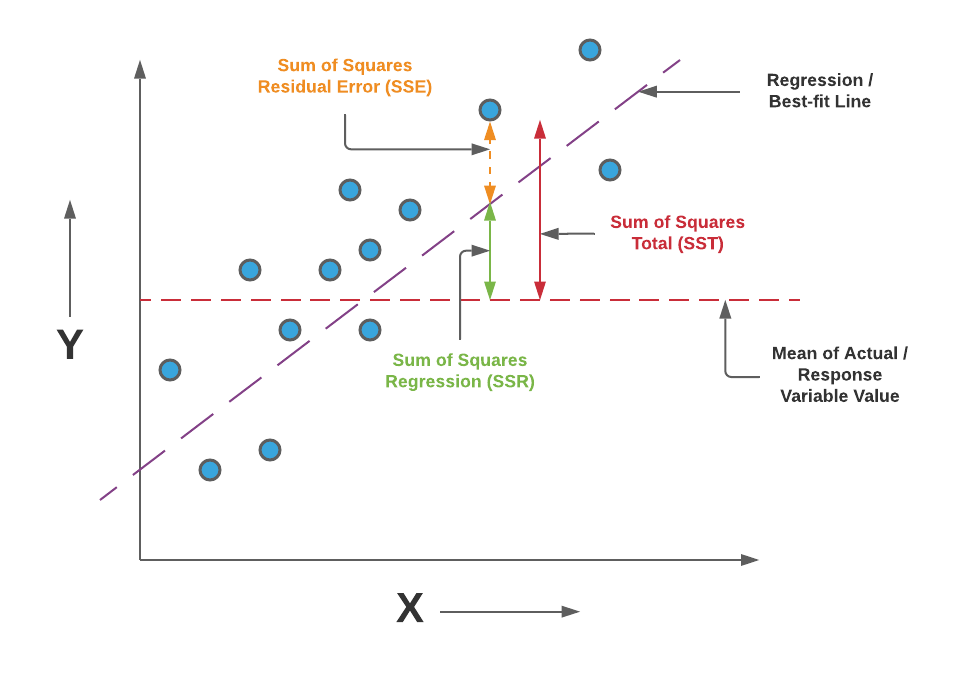
\includegraphics[width=6.04167in,height=6.14583in]{images/regression_terminologies.png}

\hypertarget{r2-thresholds}{%
\section{\texorpdfstring{\(R^{2}\)
Thresholds}{R\^{}\{2\} Thresholds}}\label{r2-thresholds}}

\(R^2 = \frac{\text{Sum of Squares Explained by Regression (SSR)}}{\text{Total Sum of Squares (before regression)(TSS)}} = \frac{\underset{i=1}{\stackrel{n}{\sum}}(\hat{y}_{i} - \overline{y})^2}{\underset{i=1}{\stackrel{n}{\sum}}(y_{i} - \overline{y})^{2}}\)

\begin{itemize}
\tightlist
\item
  The coefficient of determination can take values between 0 and 1, but
  is commonly reported as a percentage, as it represent the proportion
  of the variation in the dependent variable (\(Y_{i}\)) which is
  explained by the predictor/independent variable (\(X_{i}\)).
\item
  The higher the \(R^{2}\) value (at least \(70\%\)) the better the
  model fit.
\item
  A reasonable model fit would be more \(R^{2} >= 60\%\).
\end{itemize}

\hypertarget{exploring-the-errors}{%
\section{Exploring the Errors}\label{exploring-the-errors}}

\begin{itemize}
\item
  To assess the quality of the model further we need to look at the
  \emph{errors} or \emph{residuals} \((y_{i} - \hat{y}_{i})\) after
  running the regression model.
\item
  Model residuals should be \textbf{randomly scattered} with \textbf{no
  extreme values} and should have a \textbf{mean of zero}.
\item
  Should these requirements not be met we would have to further
  investigate whether there is information in the residuals that could
  be covered by the model or be considered a cause for concern.
\item
  A histogram of the residuals and normal probability plot can help you
  decide how well your residuals fit into the model.
\end{itemize}

\hypertarget{histogram-of-model-residuals}{%
\section{Histogram of model
residuals}\label{histogram-of-model-residuals}}

\begin{Shaded}
\begin{Highlighting}[]
\CommentTok{\# Create model for raw data}
\NormalTok{mod1 }\OtherTok{\textless{}{-}}
  \FunctionTok{lm}\NormalTok{(weight\_lbs }\SpecialCharTok{\textasciitilde{}}\NormalTok{ height\_in,}
     \AttributeTok{data =}\NormalTok{ handw)}

\CommentTok{\# Create residuals object}
\NormalTok{residuals\_df }\OtherTok{\textless{}{-}} 
\NormalTok{  mod1}\SpecialCharTok{$}\NormalTok{residuals }\SpecialCharTok{|\textgreater{}}
  \FunctionTok{as\_tibble}\NormalTok{() }\SpecialCharTok{|\textgreater{}}
  \FunctionTok{rename}\NormalTok{(}\AttributeTok{residuals =}\NormalTok{ value)}

\CommentTok{\# Plot the data}
\FunctionTok{ggplot}\NormalTok{(residuals\_df, }\FunctionTok{aes}\NormalTok{(}\AttributeTok{x =}\NormalTok{ residuals)) }\SpecialCharTok{+}
  \FunctionTok{geom\_histogram}\NormalTok{(}\AttributeTok{binwidth =} \DecValTok{10}\NormalTok{) }\SpecialCharTok{+}
  \FunctionTok{labs}\NormalTok{(}\AttributeTok{title =} \StringTok{"Histogram of Residuals"}\NormalTok{,}
       \AttributeTok{x =} \StringTok{"Residuals"}\NormalTok{,}
       \AttributeTok{y =} \StringTok{"Frequency"}\NormalTok{)}
\end{Highlighting}
\end{Shaded}

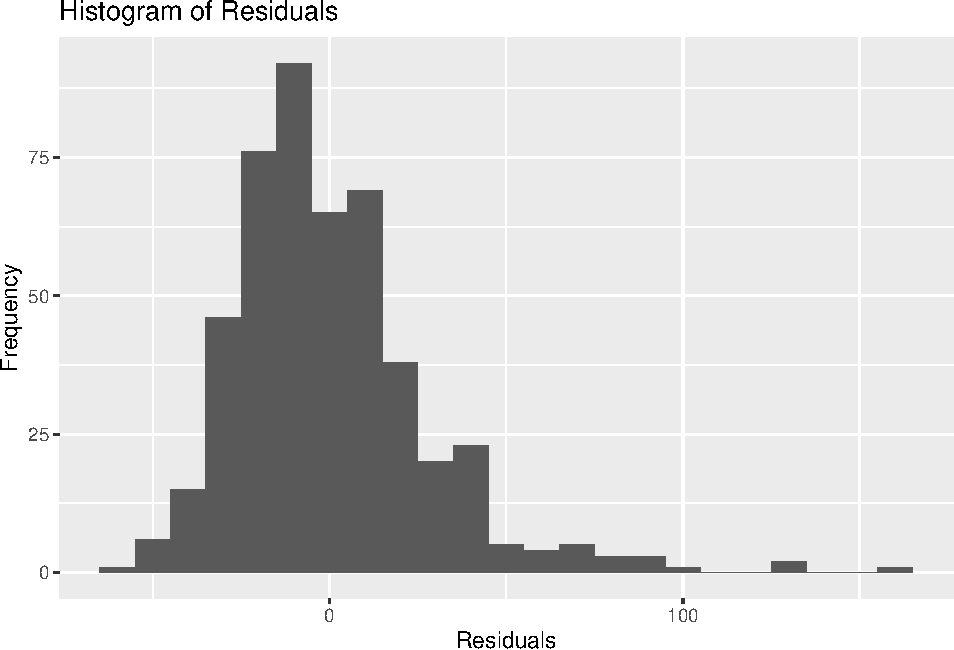
\includegraphics{L9_Regression_model_fitting_pdf_files/figure-latex/unnamed-chunk-10-1.pdf}

Are the residuals \textbf{randomly scattered} with \textbf{no extreme
values}?

\hypertarget{transformed-data-residuals-plot}{%
\section{Transformed data: residuals
plot}\label{transformed-data-residuals-plot}}

\begin{Shaded}
\begin{Highlighting}[]
\CommentTok{\# Create model for transformed data}
\NormalTok{mod2 }\OtherTok{\textless{}{-}}
  \FunctionTok{lm}\NormalTok{(wlog }\SpecialCharTok{\textasciitilde{}}\NormalTok{ hlog,}
     \AttributeTok{data =}\NormalTok{ handw\_log)}

\CommentTok{\# Create residuals object}
\NormalTok{residuals\_df }\OtherTok{\textless{}{-}} 
\NormalTok{  mod2}\SpecialCharTok{$}\NormalTok{residuals }\SpecialCharTok{|\textgreater{}}
  \FunctionTok{as\_tibble}\NormalTok{() }\SpecialCharTok{|\textgreater{}}
  \FunctionTok{rename}\NormalTok{(}\AttributeTok{residuals =}\NormalTok{ value)}

\CommentTok{\# Plot the data}
\FunctionTok{ggplot}\NormalTok{(residuals\_df, }\FunctionTok{aes}\NormalTok{(}\AttributeTok{x =}\NormalTok{ residuals)) }\SpecialCharTok{+}
  \FunctionTok{geom\_histogram}\NormalTok{(}\AttributeTok{bins =} \DecValTok{30}\NormalTok{) }\SpecialCharTok{+}
  \FunctionTok{labs}\NormalTok{(}\AttributeTok{title =} \StringTok{"Histogram of Log Transformed Residuals"}\NormalTok{,}
       \AttributeTok{x =} \StringTok{"Log(residuals)"}\NormalTok{,}
       \AttributeTok{y =} \StringTok{"Frequency"}\NormalTok{)}
\end{Highlighting}
\end{Shaded}

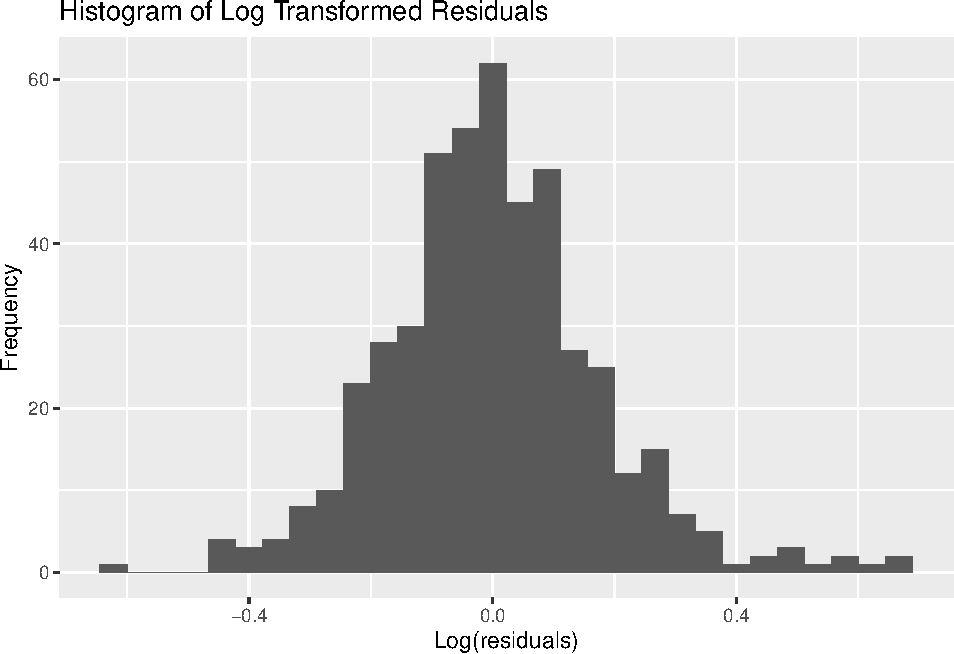
\includegraphics{L9_Regression_model_fitting_pdf_files/figure-latex/unnamed-chunk-11-1.pdf}

Are the residuals \textbf{randomly scattered} with \textbf{no extreme
values}?

\hypertarget{quantile-quantile-q-q-plot}{%
\section{Quantile quantile (Q-Q)
plot}\label{quantile-quantile-q-q-plot}}

\begin{itemize}
\tightlist
\item
  A Q-Q plot compares the quantiles of the observed data to the
  quantiles of a theoretical distribution.
\item
  It plots the observed quantiles on the y-axis and the theoretical
  quantiles on the x-axis.
\item
  The primary purpose of a Q-Q plot is to visually assess how well the
  observed data fits a specified theoretical distribution.
\end{itemize}

\begin{itemize}
\tightlist
\item
  It helps identify deviations from the theoretical distribution, such
  as skewness, kurtosis, or other anomalies.
\item
  In regression analysis and other statistical modeling, Q-Q plots are
  used to check the normality of residuals, which is an assumption for
  many statistical tests and models.
\end{itemize}

\hypertarget{interpreting-a-q-q-plot}{%
\section{Interpreting a Q-Q plot}\label{interpreting-a-q-q-plot}}

\begin{itemize}
\tightlist
\item
  If the data points lie approximately along a straight diagonal (45°)
  line, it suggests that the data follows the theoretical distribution.
\item
  Deviations from the diagonal line indicate departures from the
  theoretical distribution. For example, a systematic curve might
  indicate skewness, while points that diverge at the ends might
  indicate heavy tails.
\end{itemize}

\begin{center}\rule{0.5\linewidth}{0.5pt}\end{center}

\begin{Shaded}
\begin{Highlighting}[]
\CommentTok{\# Extract residuals}
\NormalTok{residuals }\OtherTok{\textless{}{-}}
\NormalTok{  mod1}\SpecialCharTok{$}\NormalTok{residuals}

\CommentTok{\# Calculate theoretical quantiles}
\NormalTok{mod1\_quantiles }\OtherTok{\textless{}{-}}
  \FunctionTok{qqnorm}\NormalTok{(residuals, }\AttributeTok{plot.it =} \ConstantTok{FALSE}\NormalTok{)}\SpecialCharTok{$}\NormalTok{x}

\CommentTok{\# Create a data frame with residuals and theoretical quantiles}
\NormalTok{pp\_df }\OtherTok{\textless{}{-}} 
  \FunctionTok{data.frame}\NormalTok{(}
  \AttributeTok{residuals =}\NormalTok{ residuals,}
  \AttributeTok{theoretical\_quantiles =}\NormalTok{ mod1\_quantiles}
\NormalTok{)}

\CommentTok{\# Plot the Q{-}Q plot}
\FunctionTok{ggplot}\NormalTok{(pp\_df, }\FunctionTok{aes}\NormalTok{(}\AttributeTok{sample =}\NormalTok{ residuals)) }\SpecialCharTok{+}
  \FunctionTok{stat\_qq}\NormalTok{() }\SpecialCharTok{+}
  \FunctionTok{stat\_qq\_line}\NormalTok{() }\SpecialCharTok{+}
  \FunctionTok{labs}\NormalTok{(}\AttributeTok{title =} \StringTok{"Normal Q{-}Q Plot of Residuals"}\NormalTok{,}
       \AttributeTok{x =} \StringTok{"Theoretical Quantiles"}\NormalTok{,}
       \AttributeTok{y =} \StringTok{"Sample Quantiles"}\NormalTok{) }\SpecialCharTok{+}
  \FunctionTok{theme\_minimal}\NormalTok{()}
\end{Highlighting}
\end{Shaded}

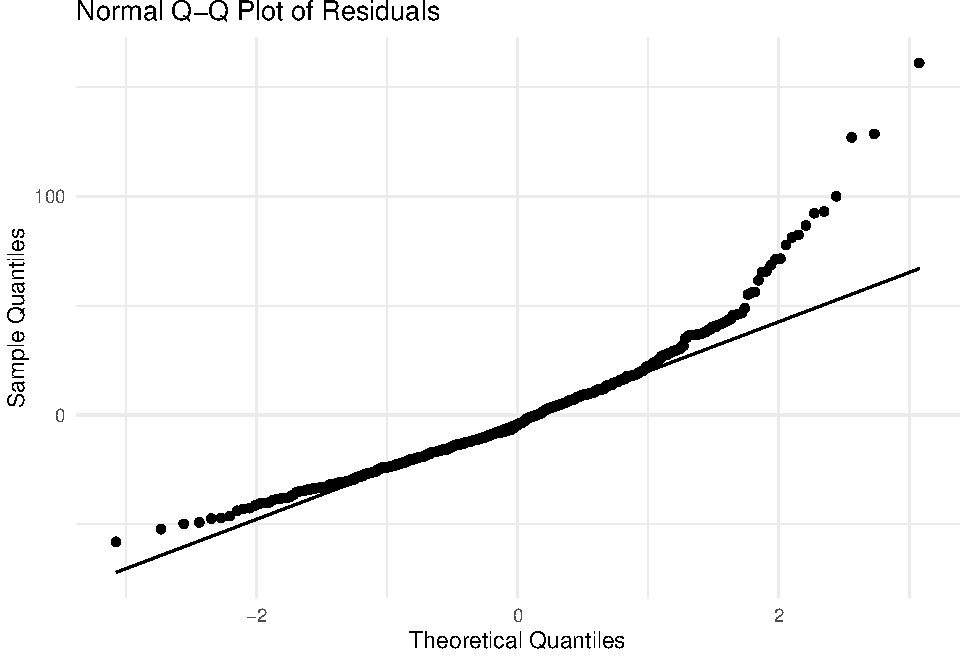
\includegraphics{L9_Regression_model_fitting_pdf_files/figure-latex/unnamed-chunk-12-1.pdf}

\hypertarget{transformed-data-normal-pp-plot}{%
\section{Transformed data: Normal PP
plot}\label{transformed-data-normal-pp-plot}}

\begin{Shaded}
\begin{Highlighting}[]
\CommentTok{\# Extract residuals}
\NormalTok{residuals }\OtherTok{\textless{}{-}}
\NormalTok{  mod2}\SpecialCharTok{$}\NormalTok{residuals}

\CommentTok{\# Calculate theoretical quantiles}
\NormalTok{mod2\_quantiles }\OtherTok{\textless{}{-}}
  \FunctionTok{qqnorm}\NormalTok{(residuals, }\AttributeTok{plot.it =} \ConstantTok{FALSE}\NormalTok{)}\SpecialCharTok{$}\NormalTok{x}

\CommentTok{\# Create a data frame with residuals and theoretical quantiles}
\NormalTok{pp\_df }\OtherTok{\textless{}{-}} 
  \FunctionTok{data.frame}\NormalTok{(}
  \AttributeTok{residuals =}\NormalTok{ residuals,}
  \AttributeTok{theoretical\_quantiles =}\NormalTok{ mod2\_quantiles}
\NormalTok{)}

\CommentTok{\# Plot the Q{-}Q plot}
\FunctionTok{ggplot}\NormalTok{(pp\_df, }\FunctionTok{aes}\NormalTok{(}\AttributeTok{sample =}\NormalTok{ residuals)) }\SpecialCharTok{+}
  \FunctionTok{stat\_qq}\NormalTok{() }\SpecialCharTok{+}
  \FunctionTok{stat\_qq\_line}\NormalTok{() }\SpecialCharTok{+}
  \FunctionTok{labs}\NormalTok{(}\AttributeTok{title =} \StringTok{"Normal Q{-}Q Plot of log(Residuals)"}\NormalTok{,}
       \AttributeTok{x =} \StringTok{"Theoretical Quantiles"}\NormalTok{,}
       \AttributeTok{y =} \StringTok{"Sample Quantiles"}\NormalTok{) }\SpecialCharTok{+}
  \FunctionTok{theme\_minimal}\NormalTok{()}
\end{Highlighting}
\end{Shaded}

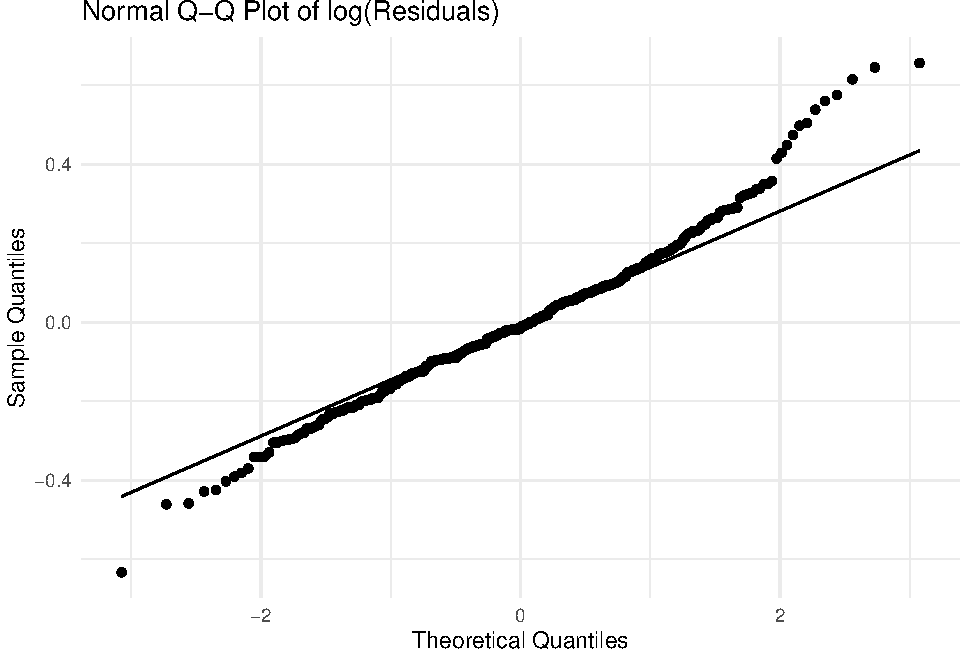
\includegraphics{L9_Regression_model_fitting_pdf_files/figure-latex/unnamed-chunk-13-1.pdf}

\hypertarget{testing-the-significance-of-the-model-and-its-coefficients}{%
\section{Testing the Significance of the model and its
coefficients}\label{testing-the-significance-of-the-model-and-its-coefficients}}

\begin{itemize}
\item
  We can use statistical tests to determine how well we are
  approximating the population parameters with those in our model. To do
  this we can use two methods:
\item
  Analysis of variance (ANOVA): tests overall significance of the model
\item
  \(t\)-test: test the individual significance of the coefficients.
\end{itemize}

\hypertarget{testing-the-overall-significance-of-the-model}{%
\section{Testing the overall significance of the
model}\label{testing-the-overall-significance-of-the-model}}

\begin{itemize}
\tightlist
\item
  Testing the overall significance of the model evaluates how well the
  independent variables reliable predict the dependent variable.
\item
  We can create hypotheses to make our statistical inferences:
\end{itemize}

\(H_{0}\): The regression model does not explain a significant
proportion of the variance in weight (our DV).

VS

\(H_{1}\): The regression model does explain a significant proportion of
the variation in weight.

And we test the above using the \(F\)-distribution.

\hypertarget{anova-for-regression-modelling}{%
\section{ANOVA for regression
modelling}\label{anova-for-regression-modelling}}

\textbf{ANOVA for regression}

\begin{longtable}[]{@{}
  >{\raggedright\arraybackslash}p{(\columnwidth - 8\tabcolsep) * \real{0.1795}}
  >{\raggedright\arraybackslash}p{(\columnwidth - 8\tabcolsep) * \real{0.1880}}
  >{\raggedright\arraybackslash}p{(\columnwidth - 8\tabcolsep) * \real{0.2137}}
  >{\raggedright\arraybackslash}p{(\columnwidth - 8\tabcolsep) * \real{0.1538}}
  >{\raggedright\arraybackslash}p{(\columnwidth - 8\tabcolsep) * \real{0.2650}}@{}}
\toprule\noalign{}
\begin{minipage}[b]{\linewidth}\raggedright
Source of Variation
\end{minipage} & \begin{minipage}[b]{\linewidth}\raggedright
Sum of Squares (SS)
\end{minipage} & \begin{minipage}[b]{\linewidth}\raggedright
Degrees of Freedom (df)
\end{minipage} & \begin{minipage}[b]{\linewidth}\raggedright
Mean Square (MS)
\end{minipage} & \begin{minipage}[b]{\linewidth}\raggedright
F-Statistic (F)
\end{minipage} \\
\midrule\noalign{}
\endhead
\bottomrule\noalign{}
\endlastfoot
Model &
\(\text{SS}_{\text{model}} = \underset{i=1}{\stackrel{n}{\sum}}(\hat{y}_i - \bar{y})^2\)
& \(k\) & \(\text{MSR} = \frac{\text{SSR}}{k}\) &
\(\frac{\text{MSR}}{\text{MSE}}\) \\
Residual &
\(\text{SS}_{\text{residual}} = \underset{i=1}{\stackrel{n}{\sum}}(y_i - \hat{y}_i)^2\)
& \(n - k - 1\) & \(\text{MSE} = \frac{\text{SSE}}{n - k - 1}\) & \\
Total &
\(\text{TSS} = SSR + SSE = \underset{i=1}{\stackrel{n}{\sum}}(y_i - \bar{y})^2\)
& \(n - 1\) & & \\
\end{longtable}

\begin{center}\rule{0.5\linewidth}{0.5pt}\end{center}

ANOVA for regression: key

\begin{itemize}
\tightlist
\item
  \(n\) = total number of observations
\item
  \(k\) = total number of independent variables
\item
  \(y\) = the observed values
\item
  \(\overline{y}\) = mean of the dependent variables
\item
  \(\hat{y}_{i}\) = the estimated values
\end{itemize}

\hypertarget{anova-for-log-transformed-model}{%
\section{ANOVA for log transformed
model}\label{anova-for-log-transformed-model}}

Remember:
\texttt{mod2\ \textless{}-\ lm(wlog\ \textasciitilde{}\ hlog,\ data\ =\ handw\_log)}

\begin{Shaded}
\begin{Highlighting}[]
\CommentTok{\# Run an ANOVA on our log transformed model}
\NormalTok{anova\_results }\OtherTok{\textless{}{-}}
  \FunctionTok{anova}\NormalTok{(mod2)}

\FunctionTok{print}\NormalTok{(anova\_results)}
\end{Highlighting}
\end{Shaded}

\begin{verbatim}
## Analysis of Variance Table
## 
## Response: wlog
##            Df  Sum Sq Mean Sq F value                Pr(>F)    
## hlog        1 182.622 182.622  5801.8 < 0.00000000000000022 ***
## Residuals 473  14.888   0.031                                  
## ---
## Signif. codes:  0 '***' 0.001 '**' 0.01 '*' 0.05 '.' 0.1 ' ' 1
\end{verbatim}

\begin{center}\rule{0.5\linewidth}{0.5pt}\end{center}

\begin{Shaded}
\begin{Highlighting}[]
\CommentTok{\# Calculate TSS}
\NormalTok{ss\_model }\OtherTok{\textless{}{-}}
\NormalTok{  anova\_results[}\StringTok{"hlog"}\NormalTok{, }\StringTok{"Sum Sq"}\NormalTok{]}

\NormalTok{ss\_residual }\OtherTok{\textless{}{-}}
\NormalTok{  anova\_results[}\StringTok{"Residuals"}\NormalTok{, }\StringTok{"Sum Sq"}\NormalTok{]}

\NormalTok{tss }\OtherTok{\textless{}{-}} 
\NormalTok{  ss\_model }\SpecialCharTok{+}\NormalTok{ ss\_residual}

\FunctionTok{print}\NormalTok{(tss)}
\end{Highlighting}
\end{Shaded}

\begin{verbatim}
## [1] 197.5102
\end{verbatim}

\hypertarget{interpreting-the-results-of-anova}{%
\section{Interpreting the results of
ANOVA}\label{interpreting-the-results-of-anova}}

\begin{itemize}
\tightlist
\item
  We can see from the output that \texttt{hlog} that the slope of the
  line is significant difference from 0, where \(p < 0.001\).
\item
  Thus we reject the null hypothesis (\(H_{0}\)).
\end{itemize}

\hypertarget{multicollinearity}{%
\section{Multicollinearity}\label{multicollinearity}}

\begin{itemize}
\tightlist
\item
  Multicollinearity occurs when \textbf{two or more predictor variables}
  in a regression model are highly correlated.
\item
  It can cause problems in estimating the coefficients of the regression
  model, leading to unreliable and unstable estimates.
\item
  High multicollinearity inflates the standard errors of the
  coefficients, making it difficult to determine the individual effect
  of each predictor.
\end{itemize}

\hypertarget{variance-inflation-factor-vif}{%
\section{Variance Inflation Factor
(VIF)}\label{variance-inflation-factor-vif}}

\begin{itemize}
\tightlist
\item
  VIF quantifies the extent of multicollinearity in a regression model.
\item
  It measures how much the variance of a regression coefficient is
  inflated due to multicollinearity.
\end{itemize}

\[\text{VIF}_{j} = \frac{1}{1 - R_{j}^2}\] - \(\text{VIF}_{j}\) = the
variance inflation factor for variable \emph{j} - \(R_{j}^2\) is the
\(R^2\) of the regression of variable \emph{j} over the rest of the
variables

\hypertarget{vif-parameters}{%
\section{VIF parameters}\label{vif-parameters}}

\begin{itemize}
\tightlist
\item
  VIF near to 1 indicate no or little correlation between predictor
  variable j and the other predictors.
\item
  VIF values above 4 suggests that multicollinearity may be inflating a
  coefficient values due to strong predictor correlations
\item
  If VIF \textgreater{} 10 then multicollinearity is serious, pointing
  to unreliable parameter estimates.
\end{itemize}

\hypertarget{checking-the-multicollinearity-of-our-grades-regressopn-model}{%
\section{Checking the multicollinearity of our grades regressopn
model}\label{checking-the-multicollinearity-of-our-grades-regressopn-model}}

\begin{Shaded}
\begin{Highlighting}[]
\CommentTok{\# Grades predicted by GPA, lectures attended, and number of VLE downloads }
\NormalTok{model }\OtherTok{\textless{}{-}} 
  \FunctionTok{lm}\NormalTok{(grade }\SpecialCharTok{\textasciitilde{}}\NormalTok{ GPA }\SpecialCharTok{+}\NormalTok{ lecture }\SpecialCharTok{+}\NormalTok{ nclicks, grades) }

\CommentTok{\# Calculate VIF values}
\NormalTok{vif\_values }\OtherTok{\textless{}{-}} 
  \FunctionTok{vif}\NormalTok{(model)}

\CommentTok{\# Display VIF values}
\FunctionTok{print}\NormalTok{(vif\_values)}
\end{Highlighting}
\end{Shaded}

\begin{verbatim}
##      GPA  lecture  nclicks 
## 1.277344 1.337824 1.183668
\end{verbatim}

\begin{center}\rule{0.5\linewidth}{0.5pt}\end{center}

What can you infer from the output?

\hypertarget{roundup}{%
\section{Roundup}\label{roundup}}

\begin{itemize}
\tightlist
\item
  Today we looked at ways to check the fit of your regression model
\item
  These are important for validating your analytical approach
\item
  When you have more than one predictor, you need to be aware of
  multicollinearity
\item
  In Thursdays lab we will begin our revision of the course.
\end{itemize}

\hypertarget{references}{%
\section*{References}\label{references}}
\addcontentsline{toc}{section}{References}

\hypertarget{refs}{}
\begin{CSLReferences}{1}{0}
\leavevmode\vadjust pre{\hypertarget{ref-Canduela_Raeside_2020}{}}%
Canduela, Jesus, and Robert Raeside. 2020. \emph{The Quantitative
Researcher}. Heriot-Watt University.
\href{https://www.hw.ac.uk/ebs}{www.hw.ac.uk/ebs}.

\end{CSLReferences}

\end{document}
